\documentclass{beamer}

\newcommand{\lesson}{Iterators}


\newcommand{\course}{Introduction to Object-Oriented Programming}
\subject{\course}
\title[\lesson]{\course}
\subtitle{\lesson}

\author[CS 1331]
{Christopher Simpkins \\\texttt{chris.simpkins@gatech.edu}}
\institute[Georgia Tech]

\date[]{}

\newcommand{\link}[2]{\href{#1}{\textcolor{blue}{\underline{#2}}}}
\newcommand{\code}{http://www.cs1331.org/code}

\usepackage{colortbl}

% If you have a file called "university-logo-filename.xxx", where xxx
% is a graphic format that can be processed by latex or pdflatex,
% resp., then you can add a logo as follows:

% \pgfdeclareimage[width=0.6in]{coc-logo}{cc_2012_logo}
% \logo{\pgfuseimage{coc-logo}}

\mode<presentation>
{
  \usetheme{Berlin}
  \useoutertheme{infolines}

  % or ...

 \setbeamercovered{transparent}
  % or whatever (possibly just delete it)
}

\usepackage{tikz}
% Optional PGF libraries
\usepackage{pgflibraryarrows}
\usepackage{pgflibrarysnakes}
\usepackage{pgfplots}
\usepackage{fancybox}
\usepackage{listings}
\usepackage{hyperref}
\hypersetup{colorlinks=true,urlcolor=blue}
\usepackage[english]{babel}
% or whatever

\usepackage[latin1]{inputenc}
% or whatever

\usepackage{times}
\usepackage[T1]{fontenc}
% Or whatever. Note that the encoding and the font should match. If T1
% does not look nice, try deleting the line with the fontenc.


\usepackage{listings}

% "define" Scala
\lstdefinelanguage{scala}{
  morekeywords={abstract,case,catch,class,def,%
    do,else,extends,false,final,finally,%
    for,if,implicit,import,match,mixin,%
    new,null,object,override,package,%
    private,protected,requires,return,sealed,%
    super,this,throw,trait,true,try,%
    type,val,var,while,with,yield},
  otherkeywords={=>,<-,<\%,<:,>:,\#,@},
  sensitive=true,
  morecomment=[l]{//},
  morecomment=[n]{/*}{*/},
  morestring=[b]",
  morestring=[b]',
  morestring=[b]""",
}

\usepackage{color}
\definecolor{dkgreen}{rgb}{0,0.6,0}
\definecolor{gray}{rgb}{0.5,0.5,0.5}
\definecolor{mauve}{rgb}{0.58,0,0.82}

% Default settings for code listings
\lstset{frame=tb,
  language=scala,
  aboveskip=2mm,
  belowskip=2mm,
  showstringspaces=false,
  columns=flexible,
  basicstyle={\scriptsize\ttfamily},
  numbers=none,
  numberstyle=\tiny\color{gray},
  keywordstyle=\color{blue},
  commentstyle=\color{dkgreen},
  stringstyle=\color{mauve},
  frame=single,
  breaklines=true,
  breakatwhitespace=true,
  keepspaces=true
  %tabsize=3
}


% If you wish to uncover everything in a step-wise fashion, uncomment
% the following command:

% \beamerdefaultoverlayspecification{<+->}


\begin{document}

\begin{frame}
  \titlepage
\end{frame}


%------------------------------------------------------------------------
\begin{frame}[fragile]{The Collections Framework}

\begin{center}
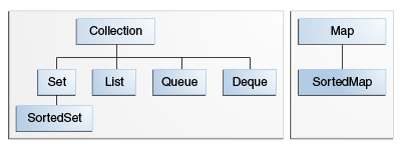
\includegraphics[width=4in]{colls-coreInterfaces.png}
\end{center}

\begin{itemize}
\item A {\it collection} is an object that represents a group of objects.
\item The collections framework allows different kinds of collections to be dealt with in an implementation-independent manner.
\end{itemize}


\end{frame}
%------------------------------------------------------------------------

%------------------------------------------------------------------------
\begin{frame}[fragile]{Collection Framework Components}

The Java collections framework consists of:
\begin{itemize}
\item Collection interfaces representing different types of collections (sets, lists, etc)
\item General purpose implementations (like {\tt ArrayList} or {\tt HashSet})
\item Absract implementations to support custom implementations
\item Algorithms defined in static utility methods that operate on collections (like {\tt Collections.sort(List<T> list)})
\item {\bf Infrastructure interfaces that support collections (like {\tt Iterator})}
\end{itemize}
Today we'll learn a few basic concepts, then tour the collections library.
\end{frame}
%------------------------------------------------------------------------

%------------------------------------------------------------------------
\begin{frame}[fragile]{The {\tt Collection} Interface}


{\tt Collection} is the root interface of the collections framework, declaring basic operations such as:
\begin{itemize}
\item {\tt add(E e)} to add elements to the collection
\item {\tt contains(Object key)} to determine whether the collection contains {\tt key}
\item {\tt isEmpty()} to test the collection for emptiness
\item {\bf {\tt iterator()} to get an interator over the elements of the collection}
\item {\tt remove(Object o)} to remove a single instance of {\tt o} from the collection, if present
\item {\tt size()} to find out the number of elements in the collection
\end{itemize}
None of the collection implementations in the Java library implement {\tt Collection} directly.  Instead they implement {\tt List} or {\tt Set}.

\end{frame}
%------------------------------------------------------------------------


%------------------------------------------------------------------------
\begin{frame}[fragile]{Iterators}


Iterators are objects that provide access to the elements in a collection.  In Java iterators are represented by the {\tt Iterator} interface, which contains three methods:
\begin{itemize}
\item {\tt hasNext()} returns true if the iteration has more elements.
\item {\tt next()} returns the next element in the iteration.
\item {\tt remove()} removes from the underlying collection the last element returned by the iterator (optional operation).
\end{itemize}

The most basic and common use of an iterator is to traverse a collection (visit all the elements in a collection):
\begin{lstlisting}[language=Java]
ArrayList tasks = new ArrayList();
// ...
Iterator tasksIter = tasks.iterator();
while (tasksIter.hasNext()) {
    Object task = tasksIter.next();
    System.out.println(task);
}
\end{lstlisting}

See \link{\code/collections/ArrayListBasics.java}{ArrayListBasics.java} for examples.

\end{frame}
%------------------------------------------------------------------------

%------------------------------------------------------------------------
\begin{frame}[fragile]{The Iterable Interface}

An instance of a class that implements the {\tt Iterable} interface can be the target of a for-each loop.  The {\tt Iterable} interface has one abstract method, {\tt iterator}:

\begin{lstlisting}[language=Java]
public interface Iterable<T> {
    Iterator<T> iterator();
}
\end{lstlisting}

Let's see how we can implement an iterator for \link{\code/collections/DynamicArray.java}{DynamicArray.java}

\end{frame}
%------------------------------------------------------------------------

%------------------------------------------------------------------------
\begin{frame}[fragile]{DynamicArray}

\link{\code/collections/DynamicArray.java}{DynamicArray.java} is like an {\tt ArrayList}

\begin{lstlisting}[language=Java]
public class DynamicArray<E> implements Iterable<E> {
    private class DynamicArrayIterator implements Iterator<E> {
        ???
    }
    private Object[] elements;
    private int lastIndex;

    public DynamicArray() { this(10); }
    public DynamicArray(int capacity) { ... }
    public Iterator<E> iterator() {return new DynamicArrayIterator();}
    public void add(E item) { ... }
    public E get(int index) { ... }
    public void set(int index, E item) { ... }
    public int size() { ... }
    public E remove(int index) { ... }
}
\end{lstlisting}

Assuming the methods above are defined, how do we write {\tt DynamicArrayIterator}?

\end{frame}
%------------------------------------------------------------------------

%------------------------------------------------------------------------
\begin{frame}[fragile]{DynamicArrayIterator}
\vspace{-.05in}
The key component of an iterator is a {\it cursor}: a pointer to the next element in the collection.
\vspace{-.05in}
\begin{itemize}
\item Since {\tt DynamicArray} uses an array as its backing data store, the cursor is simply an index into this array
\item The first element to be accessed is at index 0
\end{itemize}
\vspace{-.05in}
\begin{lstlisting}[language=Java]
public class DynamicArray<E> implements Iterable<E> {
    private class DynamicArrayIterator implements Iterator<E> {
        private int cursor = 0;

        public boolean hasNext() {
            return cursor <= lastIndex;
        }
        public E next() {
            if (!hasNext()) { throw new NoSuchElementException(); }
            E answer = get(cursor++);
            return answer;
        }
        public void remove() {
            DynamicArray.this.remove(cursor - 1);
        }
    }
    private Object[] elements;
    private int lastIndex;
\end{lstlisting}

\end{frame}
%------------------------------------------------------------------------

%------------------------------------------------------------------------
\begin{frame}[fragile]{DynamicArrayIterator's {\tt next} Method}

An {\tt Iterator}'s {\tt next} method

\begin{itemize}
\item returns the element the cursor currently points to, and
\item moves the cursor to the next element in the collection
\end{itemize}

\begin{lstlisting}[language=Java]
public class DynamicArray<E> implements Iterable<E> {
    private class DynamicArrayIterator implements Iterator<E> {
        private int cursor = 0;

        public boolean hasNext() { ... }
        public E next() {
            if (!hasNext()) { throw new NoSuchElementException(); }
            E answer = get(cursor++);
            return answer;
        }
        public void remove() { ... }
    }
    private Object[] elements;
    private int lastIndex;
\end{lstlisting}

\end{frame}
%------------------------------------------------------------------------

%------------------------------------------------------------------------
\begin{frame}[fragile]{DynamicArrayIterator's {\tt hasNext} Method}

An {\tt Iterator}'s {\tt hasNext} method

\begin{itemize}
\item is used by clients of the {\tt Iterator} to determine whether unvisited elements of the collection remain
\item for {\tt DynamicArray} we simply test whether the cursor is still a valid array index
\end{itemize}

\begin{lstlisting}[language=Java]
public class DynamicArray<E> implements Iterable<E> {
    private class DynamicArrayIterator implements Iterator<E> {
        private int cursor = 0;

        public boolean hasNext() {
            return cursor <= lastIndex;
        }
        public E next() {
            if (!hasNext()) { throw new NoSuchElementException(); }
            E answer = get(cursor++);
            return answer;
        }
        public void remove() { ... }
    }
    private Object[] elements;
    private int lastIndex;
\end{lstlisting}

\end{frame}
%------------------------------------------------------------------------

%------------------------------------------------------------------------
\begin{frame}[fragile]{DynamicArrayIterator's {\tt remove} Method}
\vspace{-.05in}
\begin{itemize}
\item removes the last element returned by the iterator
\item the only safe way to modify a collection being iterated over
\end{itemize}
We simply use the {\tt DynamicArray}'s '{\tt remove} method
\vspace{-.05in}
\begin{lstlisting}[language=Java]
public class DynamicArray<E> implements Iterable<E> {
    private class DynamicArrayIterator implements Iterator<E> {
        private int cursor = 0;
        public boolean hasNext() { return cursor <= lastIndex; }
        public E next() {
            if (!hasNext()) { throw new NoSuchElementException(); }
            E answer = get(cursor++);
            return answer;
        }
        public void remove() {
            DynamicArray.this.remove(cursor - 1);
        }
    }
\end{lstlisting}
\vspace{-.05in}
Notice the syntax for distinguishing between the enclosing class's {\tt remove} method and the inner class's {\tt remove} method.\\
What if we called the inner class's {\tt remove} method recursively?
\end{frame}
%------------------------------------------------------------------------

%------------------------------------------------------------------------
\begin{frame}[fragile]{The Iterable Interface and the For-Each Loop}

An instance of a class that implements {\tt Iterable} can be the target of a for-each loop.
\begin{lstlisting}[language=Java]
        DynamicArray<String> da = new DynamicArray<>(2);
        da.add("Stan");
        da.add("Kenny");
        da.add("Cartman");
        System.out.println("da contents:");
        for (String e: da) {
            System.out.println(e);
        }

\end{lstlisting}

See \link{\code/collections/DynamicArray.java}{DynamicArray.java} for implementation details.

\end{frame}
%------------------------------------------------------------------------

% %------------------------------------------------------------------------
% \begin{frame}[fragile]{}


% \begin{lstlisting}[language=Java]

% \end{lstlisting}

% \begin{itemize}
% \item
% \end{itemize}


% \end{frame}
% %------------------------------------------------------------------------


\end{document}
